Der generative Designprozess ist ein iterativer Kreislauf, der aus 7 Schritten besteht. Als erstes definiert der Designer mit seinem Kunden, was gebaut werden soll. In diesem Schritt werden grundlegende Kriterien festgelegt, wie im Kapitel 'Methoden' erläutert wurde. Außerdem hilft dieser Schritt dabei, das Projekt in kleinere Problemstellungen aufzuteilen und die Übersicht zu verbessern.

Hat man die Definitionsphase abgeschlossen, fängt man mit der Datensammlungsphase an. Diese Phase legt genauere Anforderungen und Parameter fest, wie beispielsweise die Materialien, die für das Produkt verwendet werden sollen, oder die Proportionen, die das Produkt haben soll. Hierbei kommt es darauf an, um welches Projekt es sich handelt. Der Designer muss am Ende dieser Phase die Grenzen kennen, die teilweise aus den Anforderungen des Kunden, aber auch aus natürlichen Umständen bestimmt werden, insbesondere bei Bauprojekten.

In der dritten Phase des Designprozesses werden die Evaluationskriterien festgelegt, anhand derer die Software die erstellten Designs bewerten soll. Diese Phase ist besonders wichtig, da sie letztendlich darüber entscheidet, ob die Software mit den gesetzten Kriterien ein gutes Design erstellen konnte. Ausgehend von diesen Kriterien werden je nach angewendeter Methode die nächsten Gruppen an Designs erstellt. Das bedeutet wiederum, dass je präziser die festgelegten Evaluationskriterien sind, desto präzisere Designs kann die Software produzieren. Diese Anforderungen erfordern eine hohe Rechenleistung, die jedoch heutzutage von Computern bewältigt werden kann. 

Die vierte Phase dient dazu ein erstes Modell zu generieren. Hierzu werden alle Daten in die Software eingetragen und die Beziehungen zwischen den Designelementen festgelegt. Hat man das bewerkstelligt kann man die Software nun das erste mal ausführen. 

Der fünfte Schritt beinhaltet dann die Evaluation der Designs seitens der Software. Diese bewertet die generierten Designs nach den Evaluationskriterien, die in Schritt drei definiert wurden. Abhängig von der Komplexität des Projekts dauert dieses Verfahren wenige Minuten bis zu mehreren Stunden oder sogar Wochen. Es ist auch nicht ungewöhnlich, dass die Software in einer Iteration mehrere Hundert Designs erstellt.

Im sechsten Schritt entfernt die Software die Designs aus einer Iteration, die bei der Evaluation schlecht abgeschnitten haben. Dadurch kann in der nächsten Iteration mit höherer Wahrscheinlichkeit ein präziseres Ergebnis generiert werden.

Im letzten Schritt werden die Designs ausgewählt, die den Vorstellungen des Kunden entsprechen. Diese werden vor der finalen Lieferung noch einmal vom Designer überarbeitet. \autocite{12} \autocite{15} \autocite*{16}


\begin{figure}[h]
  \centering
  \begin{minipage}{0.5\textwidth}
    \centering
    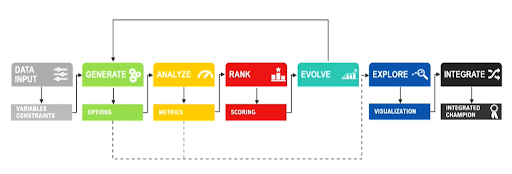
\includegraphics[width=\textwidth]{./images/7stepDesignProzess.png}
  \end{minipage}
  \caption{Generativer Designprozess Zyklus}
  \label{fig:designprozess}
\end{figure}

Mit den neuen Methoden des generativen Designs, hat sich auch die Rolle des Designers im Entwicklungsprozess geändert. \autocite*{16}